\section{Experiments}
\label{sec:experiments}

In this section, we evaluate the generative capabilities of dWorldEval and its function as an robotic policy evaluator. 
Specifically, our investigation addresses the following research questions:
\begin{itemize}
    \item \textbf{(RQ1)}
    Does dWorldEval strictly adhere to control signals, faithfully rendering execution failures from suboptimal or OOD actions rather than hallucinating outcomes?

    \item \textbf{(RQ2)}
    Does the sparse keyframe memory
    (Sec.~\ref{sec:training_history}) 
    effectively prevent spatiotemporal drift, thereby maintaining long-horizon consistency required for evaluation?

    \item \textbf{(RQ3)}
    Can the proposed Progress-as-text mechanism serve as an accurate intrinsic success metric at inference time without external oracles?

    \item \textbf{(RQ4)}
    Is dWorldEval a reliable proxy for assessing diverse robot policies? Specifically, does the performance estimated via closed-loop rollouts strongly correlate with real execution and accurately rank policies across different architectures and training stages?

    \item \textbf{(RQ5)} 
    Can the proposed $\Delta$-LPIPS metric effectively quantify action controllability and serve as a reliable diagnostic indicator for policy evaluation?
\end{itemize}


\subsection{Experimental Setup}
\label{subsec:setup}

\textbf{Platforms and data.} 
We conduct evaluations across three diverse platforms, configuring the training data for each to support world modeling:

\textbf{(1) LIBERO}~\cite{liu2024libero}:
We utilize the LIBERO-Object, LIBERO-Spatial, LIBERO-Goal, and LIBERO-100 suites with synchronized third-person and wrist views.
To enable failure-aware scoring, we augment the 5.5k official expert demonstrations with 1k failed rollouts from suboptimal policies.

\textbf{(2) RoboTwin}~\cite{mu2025robotwin}:
We select the ARX arm configuration to evaluate contact-rich tableware manipulation, yielding 5.5k trajectories across 10 tasks (e.g., multi-object stacking and precise pick-and-place).

\textbf{(3) Real-world setup}:
We deploy a physical bimanual AgileX system (Figure~\ref{fig:real_setup}) with two 6-DoF arms and three synchronized RealSense 457 cameras.
The dataset totals 5.2k trajectories (including 1k human-collected failures) across five tasks: Bussing Table, Place Cup, Handover Block, Strike Block and Place Bottles.


% \textbf{(1) LIBERO}~\cite{liu2024libero}: 
% We utilize the LIBERO-Object, LIBERO-Spatial, LIBERO-Goal, and LIBERO-100 suites, featuring synchronized third-person and wrist views. 
% To enable failure-aware scoring, we augment the 5.5k official expert demonstrations with 1k failed rollouts collected from suboptimal policies.

% \textbf{(2) RoboTwin}~\cite{mu2025robotwin}: 
% We select the ARX arm configuration to evaluate contact-rich tableware manipulation. 
% The resulting dataset comprises 5.5k trajectories across 10 distinct tasks, ranging from multi-object stacking (e.g., blocks and bowls) to precise pick-and-place operations.

% \textbf{(3) Real-world setup}: 
% We deploy a physical bimanual AgileX system, as shown in Figure~\ref{fig:real_setup}, featuring two 6-DoF arms, and recorded via three synchronized RealSense 457 cameras.
% The collected dataset totals 5.2k trajectories (including 1k human-collected failures) covering four tasks: Bussing Table, Place Cup, Handover Block, and Strike Block.

\textbf{Baselines and target policies.} 
We benchmark dWorldEval against video diffusion baselines including WorldEval~\cite{li2025worldeval}, WorldGym~\cite{quevedo2506worldgym} and Ctrl-World~\cite{guo2025ctrl}. ensuring identical training data splits for fair comparison. 
And we assess its capabilities across varied policies: multiple training checkpoints of a base policy ($\pi_0$~\cite{[pi0}) on LIBERO, and heterogeneous architectures (e.g., DexVLA~\cite{wen2025dexvla}, Diffusion Policy~\cite{diffusion-policy}) across RoboTwin and real-world environments.


\begin{figure*}[t]
    \centering
    
\includegraphics[width=0.9\textwidth]{figures/fail_success_robotwin.pdf}
    \caption{\textbf{Visualization of ground-truth vs.\ generated multi-view rollouts on RoboTwin}~\cite{mu2025robotwin}.
    \textbf{Left/Right}: suboptimal vs.\ successful execution.
    \textbf{Top/Bottom}: ground-truth simulator rollout vs.\ dWorldEval prediction, conditioned on identical action sequences. 
    Each sequence displays the initial state followed by synchronized future frames.}
    \label{fig:fail_success_robotwin}
\end{figure*}


\textbf{Implementation details.} 
All models predict multi-view outcomes at $256^2$ resolution, conditioned on a sparse history of $K=4$ keyframes ($128^2$). 
Regarding the loss weights in Eq.~\ref{eq:loss_total}, we set $w_j = 2$ for progress tokens and $w_j = 1$ for visual tokens.
The prediction horizon $\Delta$ aligns with the action chunk length (selected from $[2, 8]$). 
During inference, we employ 16-step iterative parallel decoding.


\begin{figure*}[t]
    \centering
    
\includegraphics[width=\textwidth]{figures/consistency.pdf}
    \caption{\textbf{(a) Action-controllability under suboptimal inputs.}
    We condition all methods on an unseen action sequence and compare their rollouts.
    While WorldGym~\cite{li2025worldeval} self-corrects the missed grasp into a successful pickup and WorldEval~\cite{li2025worldeval} hallucinates non-existent objects, Ctrl-World~\cite{guo2025ctrl} fails to align with the input actions.
    In contrast, dWorldEval faithfully reproduces the failure.
    \textbf{(b) Long-horizon round-trip consistency.}
    We apply a reversible action trajectory: forward actions up to $t=H\Delta$, followed by the corresponding inverse actions to $t=2H\Delta$.
    The full model returns close to the initial observation at $t=0$, whereas removing history causes accumulated drift over the round trip.}
    \label{fig:consistency}
\end{figure*}

\begin{figure*}[t]
    \centering
    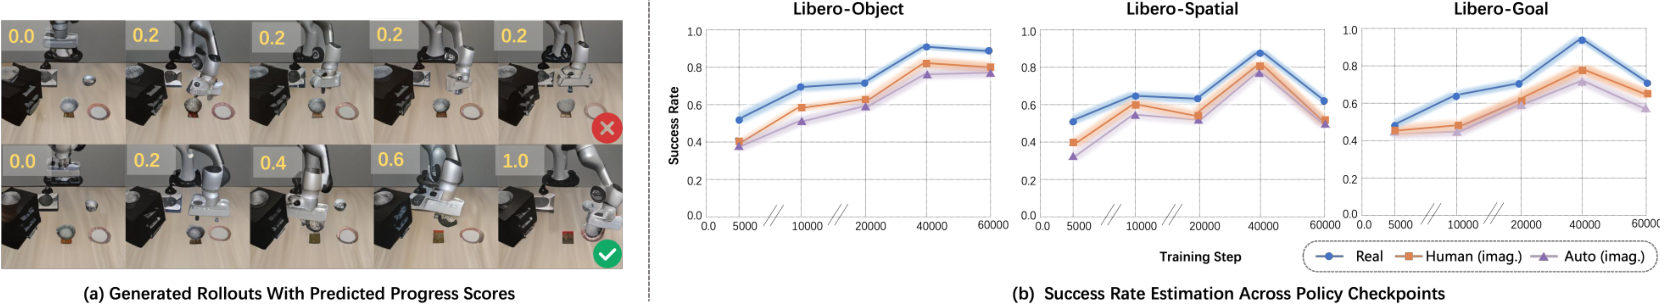
\includegraphics[width=0.98\textwidth]{figures/score_curve.pdf}
    \caption{\textbf{Joint generation enables automatic policy scoring.}
    \textbf{(a)} At each rollout step, the world model jointly predicts the future observation $\hat{o}_{t+\Delta}$ and a scalar progress score $\hat{v}_{t+\Delta}\!\in[0,1]$, which finally indicates task success or failure.
    \textbf{(b)} Success rate estimates across checkpoints of a base policy $\pi_0$~\cite{[pi0} on three LIBERO~\cite{liu2024libero} suites.
    We compare ground-truth execution (\emph{Real}) against evaluations on generated rollouts: human judgment based on the generated observations (\emph{Human}) and automatic evaluation determined by the model's predicted progress score (\emph{Auto}).}
    \label{fig:score_curve}
\end{figure*}


\begin{figure*}[t]
    \centering
    
\includegraphics[width=0.98\textwidth]{figures/corr.pdf}
    \caption{\textbf{Correlation between real-execution and world-model success rates.}
    Scatter plots compare real success rates (x-axis) against generated estimates (y-axis), reporting Pearson correlation $r$ and rank-violation \textsc{MMRV} (lower is better).
    \textbf{(a)} Comparison with video diffusion baselines (WorldEval~\cite{li2025worldeval}, WorldGym~\cite{quevedo2506worldgym} and Ctrl-World~\cite{guo2025ctrl}) on LIBERO~\cite{liu2024libero} (Single-view).
    \textbf{(b-d)} Ablation studies comparing dWorldEval against its \textit{w/o-history} variant across diverse settings:
    \textbf{(b)} LIBERO (Multi-view),
    \textbf{(c)} Robotwin~\cite{mu2025robotwin} with heterogeneous policies ($\pi_0$~\cite{[pi0}, DexVLA~\cite{wen2025dexvla}, DP~\cite{diffusion-policy}), and
    \textbf{(d)} Real-world tasks.
    dWorldEval consistently achieves superior correlation and ranking accuracy across all domains.}
    \label{fig:policy_corr}
\end{figure*}


\subsection{Evaluating the World Model}
\label{sec:wm_eval}

\subsubsection{Evaluating Action Controllability}
\label{sec:action_controllability_exp}

\paragraph{Evaluation protocol.}
To assess action controllability (RQ1), we employ a protocol on a test set constructed from two distinct interaction types:
(1) Expert success ($\mathcal{D}_{\text{succ}}$): successful trajectories collected from a fully trained policy;
(2) Suboptimal failure ($\mathcal{D}_{\text{fail}}$): failure rollouts collected from undertrained checkpoints.
We perform generation conditioned on ground-truth action sequences and evaluate on the shared third-person view.

\textbf{Evaluation metric.}
Standard LPIPS captures only static appearance. To explicitly evaluate action controllability, we introduce \textbf{$\Delta$-LPIPS}, which measures the perceptual fidelity of state transitions rather than absolute states. For a fixed stride $\Delta$, we compute difference images $\Delta o_t = o_{t+\Delta} - o_t$ (analogously for predictions $\Delta \hat{o}_t$) and define:
\begin{equation}
  \Delta\mathrm{LPIPS} = \mathbb{E}_{t}\Big[d_{\mathrm{lpips}}\big(\mathrm{norm}(\Delta \hat{o}_t), \mathrm{norm}(\Delta o_t)\big)\Big],
\end{equation}
where $\mathrm{norm}(\cdot)$ denotes per-sample RMS normalization for stability. We use $\Delta$LPIPS as our primary indicator for action-conditioned dynamic fidelity (see Sec.~\ref{sec:more_experiments} for further validation of its diagnostic correlation).

\paragraph{Experimental results.}
This visual fidelity is quantified in Tab.~\ref{tab:wm_lpips}, which exposes a critical divergence: baselines suffer severe degradation on the Failure subset (e.g., WorldGym $\Delta$LPIPS spikes from 0.347 to 0.650), whereas dWorldEval maintains consistent performance. This quantitative degradation manifests visually in Fig.~\ref{fig:consistency}(a), where baselines frequently fail to adhere to the input actions.
To verify these results stem from action controllability, we find that randomly shuffling actions (App.~\ref{app:action_shuffle}) significantly degrades $\Delta$LPIPS, proving our model is sensitive to the input actions.


\begin{table}[t]
    \centering
    
    % 左侧表格：Action controllability
    \begin{minipage}[t]{0.48\textwidth}
        \centering
        \small
        \setlength{\tabcolsep}{8pt} % 稍微调小一点列间距以确保不超宽
        \caption{\textbf{Action controllability on LIBERO}~\cite{liu2024libero}. Comparison of LPIPS vs. our dynamic-aware $\Delta$LPIPS on Expert ($\mathcal{D}_{\text{succ}}$) and Failure ($\mathcal{D}_{\text{fail}}$) subsets. Baselines degrade on failure data, while ours remains robust.}
        \label{tab:wm_lpips}
        \begin{sc}
            \begin{tabular}{lccc} 
                \toprule
                \multirow{2}{*}{Method} & LPIPS & \multicolumn{2}{c}{$\Delta$LPIPS ($\downarrow$)} \\
                \cmidrule(lr){3-4} 
                 & ($\downarrow$) & Expert & Failure \\
                \midrule
                WorldEval & 0.262 & 0.423 & 0.701 \\
                WorldGym  & 0.218 & 0.347 & 0.650 \\
                Ctrl-World  & 0.220 & 0.334 & 0.416 \\
                \midrule
                \textbf{Ours} & \textbf{0.215} & \textbf{0.315} & \textbf{0.352} \\
                \bottomrule
            \end{tabular}
        \end{sc}
    \end{minipage}%
    \hfill 
    % 右侧表格：Long-horizon consistency
    \begin{minipage}[t]{0.48\textwidth}
        \centering
        \small
        \setlength{\tabcolsep}{2.4pt} % 稍微调小一点列间距以确保不超宽
        \caption{\textbf{Long-horizon consistency analysis.} We report the round-trip LPIPS ($\downarrow$) error, averaged across all synchronized views, over varying horizons $H$. Without memory, the model suffers from progressive drift; with memory, spatiotemporal consistency is effectively preserved even at $H=20$.}
        \label{tab:h_scan_consistency}
        \begin{sc}
            \begin{tabular}{lcccc}
            \toprule
            \multirow{2}{*}{Method} & \multicolumn{4}{c}{Action Horizon ($H$)} \\
            \cmidrule(lr){2-5}
             & 5 & 10 & 15 & 20 \\
            \midrule
            Ours (W/O Memory) & 0.177 & 0.186 & 0.302 & 0.411 \\
            \textbf{Ours (Full)} & \textbf{0.130} & \textbf{0.145} & \textbf{0.193} & \textbf{0.243} \\
            \bottomrule
            \end{tabular}
        \end{sc}
    \end{minipage}
    
\end{table}

\subsubsection{Evaluating Spatiotemporal Consistency}
\label{sec:exp_consistency}

\paragraph{Evaluation protocol and metrics.}
To assess long-horizon stability (RQ2), we employ a variable-horizon round-trip protocol. We perform rollouts of length $2H$ by appending inverse actions to trajectories of varying lengths $H \in \{5, 10, 15, 20\}$. Consistency is measured via LPIPS  between the initial $o_t$ and final $\hat{o}_{t+2H}$.
We focus on memory ablation here. Baselines are detailed in Appendix~\ref{app:baseline_consistency}, as their inability to strictly follow actions  renders the round-trip metric unreliable for direct comparison.


\paragraph{Experimental results.}
Fig.~\ref{fig:consistency}(b) visualizes the cumulative drift isolated by removing memory.
This is quantified in Tab.~\ref{tab:h_scan_consistency}: while ablation errors accumulate as $H$ extends to 20, the full model maintains high fidelity (LPIPS $0.21$), confirming that keyframe memory effectively bounds long-term drift. This stability is vital: Sec.~\ref{sec:policy_eval} shows that drift leads to false negatives, severing the correlation with real-world performance.

\subsubsection{Joint subgoal-and-progress prediction enables automatic visual grading}
\label{sec:joint_progress}

\textbf{Evaluation protocol.}
We leverage the failure-augmented training regime (Sec.~\ref{subsec:setup}) to validate whether the learned progress tokens can serve as an intrinsic metric (RQ3). 
We evaluate multiple checkpoints of a base policy $\pi_0$ across four LIBERO suites and compare three success estimators:
(1) \textbf{Real}: Ground-truth success rates measured by real execution;
(2) \textbf{Human (imag.)}: Manual grading of the final generated frame;
(3) \textbf{Auto (imag.)}: Our proposed automated metric. For each imagined rollout, we examine the predicted progress token $\hat{v}_{T}$ at the final time step. The rollout is classified as successful only if this terminal score equals 1.

\paragraph{Experimental results.} As shown in Fig.~\ref{fig:score_curve}(a), the progress score is discriminative, exhibiting sharp transitions upon task completion. Crucially, Fig.~\ref{fig:score_curve}(b) demonstrates that Auto (imag.) closely tracks real execution, capturing even non-monotonic fluctuations (e.g., performance dips in later checkpoints).
This alignment closely matches human judgment. It confirms that dWorldEval bases its score on the actual visual changes, rather than simply assuming progress increases over time. This ensures the reliability of our automatic evaluation.

\subsection{World-Model as a Reliable Proxy for Policy Evaluation}
\label{sec:policy_eval}

For the ablation without memory, the generated video often suffers from severe drift, making the predicted progress token unreliable. To ensure a fair comparison, we ignore the progress and judge success  based on the generated image.

\textbf{Comparison with baselines on LIBERO.}
Fig.~\ref{fig:policy_corr}(a) evaluates policy ranking accuracy on LIBERO tasks under the single-view setting.
Existing baselines (WorldGym, WorldEval and Ctrl-World) exhibit weaker correlations and higher rank violations (MMRV up to 0.039) due to insufficient action controllability.
In contrast, dWorldEval achieves a strong linear correlation with minimal rank violation (MMRV=0.013), confirming that action-faithful generation is a prerequisite for reliable evaluation.

\textbf{Ranking heterogeneous policies across domains.} 
We further assess robustness across multi-view settings, heterogeneous architectures (RoboTwin), and physical environments (Real World).
As shown in Fig.~\ref{fig:policy_corr}(b-d), the \textit{w/o-history} ablation suffers from significant performance degradation, particularly in the multi-view setting ($r$ drops to 0.786).
In contrast, by preserving spatiotemporal consistency, dWorldEval achieves high correlations with actual execution success rates across LIBERO multi-view ($r=0.910$), Robotwin ($r=0.927$), and real-world ($r=0.918$) tasks.

\begin{table}[t]
    \centering
    
    % 左侧表格：Universal multi-view fidelity
    \begin{minipage}[t]{0.5\textwidth}
        \vspace{0pt} % 保证绝对顶部对齐
        \centering
        \small
        \setlength{\tabcolsep}{3pt} % 稍微缩小列间距以适应单栏的一半宽度
        \caption{\textbf{Universal multi-view fidelity.} Quantitative evaluation across diverse platforms (LIBERO~\cite{liu2024libero}, RoboTwin~\cite{mu2025robotwin}, Real-Robot) and synchronized viewpoints. dWorldEval maintains consistent high fidelity (low $\Delta$LPIPS) on both simulation and real-world data.}
        \label{tab:uni_fidelity}
        \begin{sc}
            \begin{tabular}{ll|cc}
                \toprule
                Dataset & Viewpoint & LPIPS ($\downarrow$) & $\Delta$LPIPS ($\downarrow$) \\
                \midrule
                \multirow{2}{*}{LIBERO} & 3rd-Person & 0.215 & 0.324 \\
                                        & Wrist & 0.192 & 0.303 \\
                \midrule
                \multirow{2}{*}{RoboTwin} & Top-Down & 0.199 & 0.317 \\
                                          & Wrist & 0.220 & 0.345 \\
                \midrule
                \multirow{2}{*}{Real World} & Top-Down & 0.272 & 0.365 \\
                                            & Wrist & 0.254 & 0.336 \\
                \bottomrule
            \end{tabular}
        \end{sc}
    \end{minipage}%
    \hfill
    % 右侧表格：Full consistency comparison
    \begin{minipage}[t]{0.46\textwidth}
        \vspace{0pt} 
        \centering
        \small 
        \renewcommand{\arraystretch}{1} 
        \setlength{\tabcolsep}{6pt}
        \caption{\textbf{Full consistency comparison.} We report the round-trip LPIPS ($\downarrow$) error averaged over varying horizons $H$. Comparisons with WorldEval~\cite{li2025worldeval}, WorldGym~\cite{quevedo2506worldgym} and Ctrl-World~\cite{guo2025ctrl}, demonstrate that our model maintains superior spatiotemporal consistency, whereas baselines suffer from significant drift.}
        \label{tab:baseline_consistency_full}
        \begin{sc}
            \begin{tabular}{lcccc}
                \toprule
                \multirow{2}{*}{Model} & \multicolumn{4}{c}{Action Horizon ($H$)} \\
                \cmidrule(lr){2-5}
                 & 5 & 10 & 15 & 20 \\
                \midrule
                WorldEval    & 0.216 & 0.320 & 0.467 & 0.531 \\
                WorldGym   & 0.191 & 0.224 & 0.308 & 0.482 \\
                Ctrl-World   & 0.149 & 0.233 & 0.296 & 0.370 \\
                \textbf{Ours (Full)} & \textbf{0.130} & \textbf{0.145} & \textbf{0.193} & \textbf{0.243} \\
                \bottomrule
            \end{tabular}
        \end{sc}
    \end{minipage}
\end{table}



\subsection{More Experiments and Ablation Study}
\label{sec:more_experiments}

\textbf{Universal fidelity across diverse platforms.} 
We provide a comprehensive assessment of visual fidelity across diverse platforms.
% , extending our analysis to RoboTwin and physical robot setups.
As detailed in Tab.~\ref{tab:uni_fidelity}, dWorldEval maintains consistently low $\Delta$LPIPS scores ($\approx 0.31$-$0.36$) across varying camera configurations and robot morphologies. 
Notably, the performance in the real-world setup remains comparable to simulation results. This consistency suggests that our unified tokenization is robust against domain gaps, maintaining high fidelity across diverse environments.


\textbf{Comparison of long-horizon consistency.} While Sec.~\ref{sec:exp_consistency} focused on memory ablation, here we benchmark against video diffusion baselines.
As detailed in Tab.~\ref{tab:baseline_consistency_full}, baselines suffer from severe inconsistency that worsens as the horizon extends.
We interpret this degradation as a compound failure: since baselines frequently ignore control signals (as established in Sec.~\ref{sec:action_controllability_exp}), their high LPIPS errors stem not only from spatiotemporal drift but also from insufficient action controllability, where the model fails to follow the action sequence.
In contrast, dWorldEval maintains high spatiotemporal consistency. Qualitative visualizations of these failure modes are provided in Appendix~\ref{app:baseline_consistency}.

